% Project report main tex file
\documentclass[11pt, a4paper]{report} 

% ----------------------------------------------------------------------
% Preamble
% ----------------------------------------------------------------------

% Packages - add any packages that you use here
\usepackage[utf8]{inputenc}
\usepackage[margin=2cm]{geometry}
\usepackage{graphicx}
\usepackage{amsmath}
\usepackage{amssymb}
\usepackage{hyperref}
\usepackage{parskip}
\usepackage{float}
\usepackage{booktabs}
\usepackage{caption}
\usepackage{lipsum}

% Use double line spacing
\usepackage{setspace}
\doublespacing

% Referencing package and options
\usepackage[
  backend=bibtex,
  citestyle=authoryear,
  bibstyle=authoryear,
  maxcitenames=2]{biblatex}
\addbibresource{references.bib}
\DeclareNameAlias{sortname}{last-first}
\setlength\bibitemsep{1em}

% Code listings packages and style
\usepackage{listings}
\usepackage{xcolor}
\lstdefinestyle{matlabcode}{
  backgroundcolor=\color{gray!10},
  commentstyle=\color{green!50!black},
  keywordstyle=\color{blue},
  stringstyle=\color{magenta},
  basicstyle=\linespread{1}\ttfamily,
  numberstyle=\tiny,
  breakatwhitespace=false,
  breaklines=true,
  captionpos=t,
  frame=single,
  keepspaces=true,
  language=matlab,
  numbers=none,
  numbersep=5pt,
  showspaces=false,
  showstringspaces=false,
  showtabs=false,
  tabsize=2,
  aboveskip=1em,
  belowskip=1em,
  belowcaptionskip=12pt
}

% Headers and footers
\usepackage{fancyhdr}
\pagestyle{fancy}
\renewcommand{\chaptermark}[1]{\markboth{\chaptername\ \thechapter.\ #1}{}}
\renewcommand{\sectionmark}[1]{\markright{\thesection.\ #1}}
\lhead{}
\rhead{\leftmark}
\setlength{\headheight}{14.5pt}
\renewcommand{\headrulewidth}{0.3pt}

% ----------------------------------------------------------------------
% Your details - enter your details here
% ----------------------------------------------------------------------
\newcommand{\myname}{Your Name}
\newcommand{\mycourse}{BSc. (Hons) Mathematics}
% \newcommand{mycourse}{BSc. (Hons) Financial Mathematics}
% \newcommand{mycourse}{MMath. (Hons) Mathematics}
\newcommand{\projecttitle}{Project Title}
\newcommand{\publishdate}{April 2020}

% ----------------------------------------------------------------------
% Document
% ----------------------------------------------------------------------
\begin{document}

% ----------------------------------------------------------------------
% Title page - shouldn't need to change this
% ----------------------------------------------------------------------
\thispagestyle{empty}
\begin{center}
  \vspace*{2cm}
  {
\includegraphics[width = 7cm]{Images/Manchester_Met_University_Horizonal_black_logo} \par}
  \vspace{1cm}
  {\bfseries\LARGE Faculty of Science and Engineering \par}
  \vspace{1cm}
  {\bfseries\Huge \myname \par}
  {\bfseries\Large \mycourse \par}
  \vspace{1cm}
  {\bfseries\Huge \projecttitle \par}
  \vspace{1cm}
  {\bfseries\Large \publishdate \par}
  \vfill
  {\bfseries\Large Department of Computing and Mathematics \par}
  \vspace{1cm}
\end{center}

% ----------------------------------------------------------------------
% Top matter
% ----------------------------------------------------------------------
\pagenumbering{roman}
\setcounter{page}{0}

% Abstract
\chapter*{Abstract}
\lipsum[1-2]      % creates dummy text

% Plagiarism disclaimer
\chapter*{Plagiarism Declaration}
With the exception of any statement to the contrary, all the material presented in this report is the result of my own efforts. In addition, no parts of this report are copied from other sources. I understand that any evidence of plagiarism and/or the use of unacknowledged third party materials will be dealt with as a serious matter.

\vspace{2cm}
Signed: \hspace{1cm} \includegraphics[width=2cm]{example-image} % change to your signature

% Acknowledgements
\chapter*{Acknowledgements}
\lipsum[3]

% Contents page, list of figures, list of tables, list of listings
\setcounter{tocdepth}{2}
\tableofcontents
\listoffigures
\listoftables
\lstlistoflistings    % comment out if not needed

% ----------------------------------------------------------------------
% Main matter
% ----------------------------------------------------------------------
\newpage
\setcounter{page}{0}
\pagenumbering{arabic}

% ----------------------------------------------------------------------
% Chapter 1
% ----------------------------------------------------------------------
\chapter{Chapter Heading} % enter the name of the chapter here
\label{cha:chapter label} % enter the chapter label here (for cross referencing)

\lipsum[1]  % creates dummy text

\section{Section Heading} % enter the name of the section here
\label{sec:section label} % enter the section label here (for cross referencing)

\lipsum[2]  % creates dummy text
 
\subsection{Subsection Heading} %enter the name of the subsection here
\label{sec:subsection label} % enter the subsection label here (for cross referencing)

\lipsum[3]  % creates dummy text

\subsection{Some maths}

\LaTeX\ is very good at presenting mathematics.

Inline equation: $ax^2 + bx + c = 0$

Display equation:
$$x = \frac{-b \pm \sqrt{b^2 - 4ac}}{2a}$$

Numbered equation:
\begin{align}
  \label{eq:equation label} % enter the equation label here (for cross referencing)
  \frac{\partial}{\partial t} U + \nabla \cdot F = 0
\end{align}

Aligned equation (equals signs line up)
\begin{align}
  \notag % means the current line will not be numbered
  \label{eq:dot product}
  \mathbf{a} \cdot \mathbf{b} &= \sum_{i=1}^n a_ib_i \\
  &= a_1b_1 + a_2b_2 + \cdots + a_nb_n
\end{align}

Aligned equation with no numbers
\begin{align*}
  \mathbf{a} \times \mathbf{b} &= \begin{vmatrix} 
  \mathbf{i} & \mathbf{j} & \mathbf{k} \\ a_1 & a_2 & a_3 \\ b_1 & b_2 & b_3 \end{vmatrix} \\
  &= \mathbf{i}(a_2b_3 - a_3b_2) - \mathbf{j}(a_1b_3 - a_3b_1) + \mathbf{k}(a_1b_2 - a_2b_1)  
\end{align*}

\section{Figures and tables}

\begin{figure}[H]
  \begin{center}
    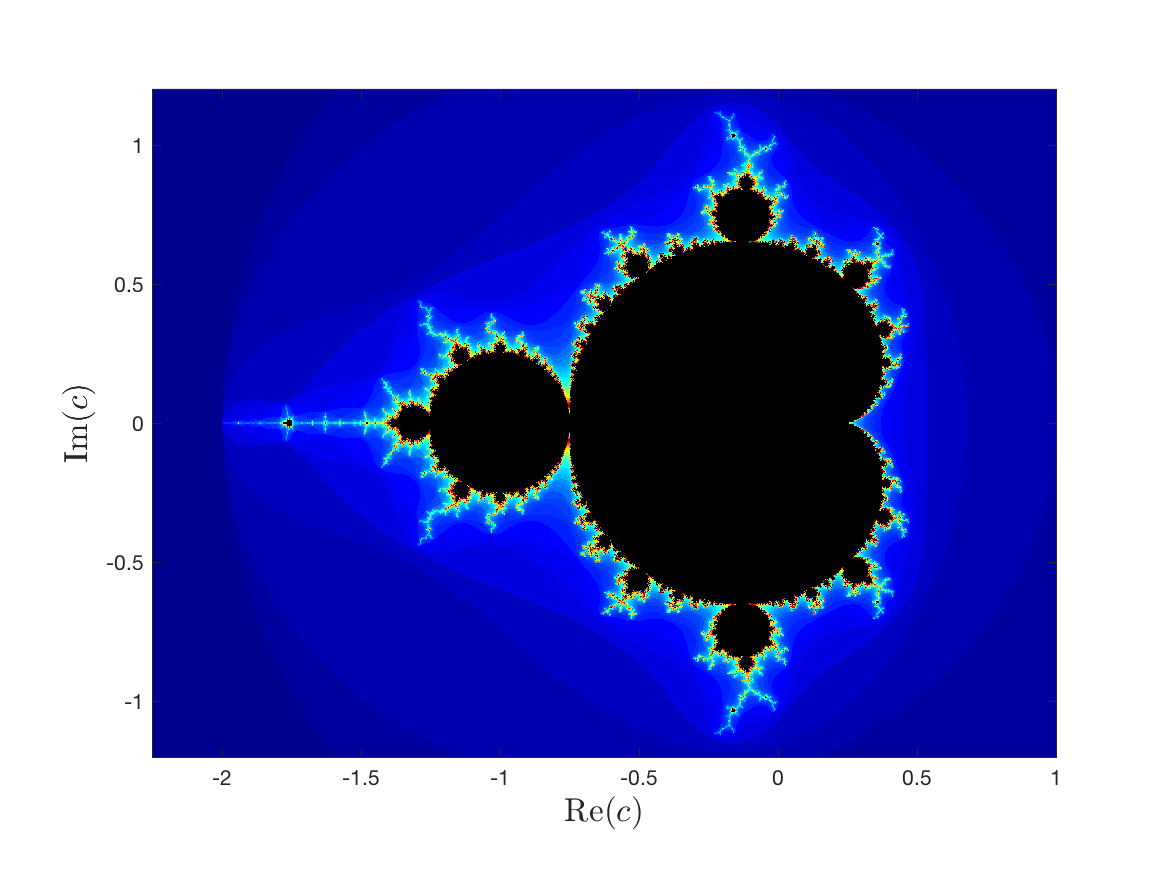
\includegraphics[width = 0.6\textwidth]{Images/mandelbrot} % enter the filename here
    \caption{This is a figure caption, note how it appears underneath the figure.} % enter the figure caption here
    \label{fig:figure label} % enter the figure label here (for cross referencing)
  \end{center}
\end{figure}


\begin{table}[H]
  \caption{This is a table caption, not how it appears above the table.}
  \label{tab:table label} % enter the table label here (for cross referencing)
  \begin{center}
    \begin{tabular}{lcr} % three columns aligned left, centre and right respectively
      \toprule % thick horizontal line at the top of the table
      first column & second column & third column \\
      \midrule % single horizontal line separating the column headings
      This & This & This \\
      column & column & column \\
      is left & is centrally & is right \\
      aligned & aligned & aligned \\
      \bottomrule % thick horizontal line at the bottom of the table
    \end{tabular}
  \end{center}
\end{table}

\subsection{Program code}

\begin{lstlisting}[style=matlabcode,
    caption = A MATLAB function to compute the first $n$ numbers of the Fibonacci series,
    label = mat:fibonacci
    ]
function y = fibonacci(n)

% This function calculates the first n terms in the Fibonacci series

y(1) = 0;
y(2) = 1;

for i = 3 : n
    y(i) = y(i-2) + y(i-1)
end

end
\end{lstlisting}

\section{Referencing}
References can be cited so that the author names(s) are a part of the sentence, e.g., \textcite{stroud:2013}, \textcite{harten:1983}

Alternatively, references can be cited so that the author names appear in the brackets (for when the name of the author is not relevant to the sentence), e.g., \parencite{stroud:2013},  \parencite{harten:1983}.

Cross referencing is easily done by using the label of the item you are referencing to (see source code for details).
\begin{itemize}
  \item Chapter~\ref{cha:chapter label}
  \item Section~\ref{sec:section label}
  \item Eq.~(\ref{eq:equation label}
  \item Table~\ref{tab:table label}
  \item Fig.~\ref{fig:figure label}
  \item Page~\pageref{eq:equation label}
\end{itemize}

Above is an example of an itemised (or bulleted) list. You can also create numbered lists:
\begin{enumerate}
  \item First list item
  \item Second list item
  \begin{enumerate}
    \item First sub list item
    \item Second sub list item
  \end{enumerate}
  \item Third list item
\end{enumerate}

% ----------------------------------------------------------------------
% Chapter 2
% ----------------------------------------------------------------------
\chapter{Another Chapter Heading} % enter the name of the chapter here
\label{cha:chapter 2 label} % enter the chapter label here (for cross referencing)

% Add more chapters in a similar manner

% ----------------------------------------------------------------------
% Reference list (shouldn't need to change this)
% ----------------------------------------------------------------------
\addcontentsline{toc}{chapter}{References}
\renewcommand\bibname{References}
\printbibliography

% ----------------------------------------------------------------------
% Appendices
% ----------------------------------------------------------------------
\appendix
\chapter{Appendix Chapter}

\section{Appendix section}
\lipsum[4]  % creates dummy text

\chapter{Another Appendix Chapter}
\lipsum[5]  % creates dummy text

% end document
\end{document}